\section{Auswertung}
In diesem Kapitel sollen die aufgenommenen Messwerte Ausgewertet und verrechnet werden.

  \begin{figure}
    \centering
    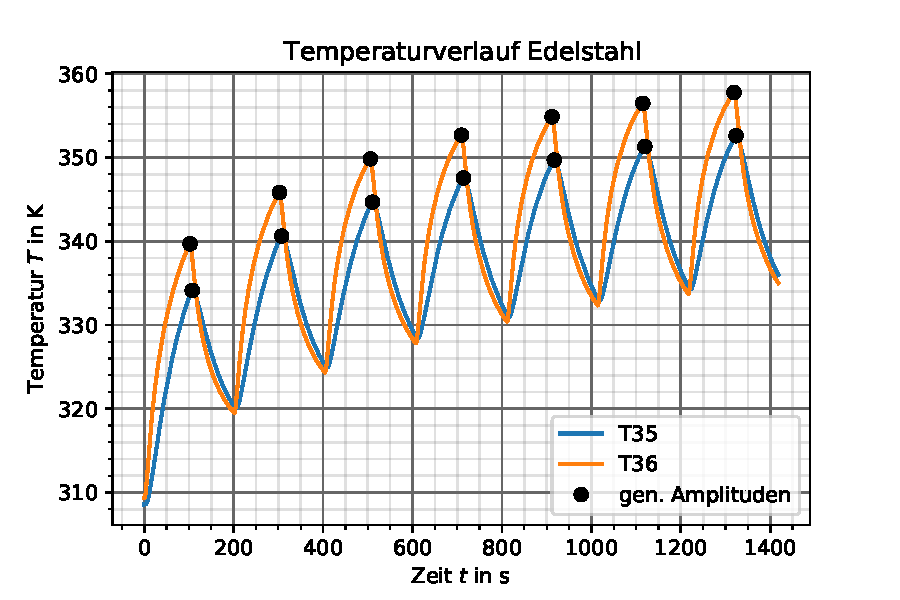
\includegraphics{welleedelstahl.pdf}
    \caption{Temperaturverlauf von Edelstahl im Angström-Verfahren zu sehen.}
    \label{fig:edelwelle}
  \end{figure}
 
  
\begin{table}
    \centering
      \caption{Die Ergebnisse der Rechnungen.}
      \label{tab:ergebnisse}
      \sisetup{table-format=1.2}
      \begin{tabular}{S[table-format=3.2] S S S S S [table-format=3.2]}
        \toprule
        {Material}&{ $T$ / s}&{ $\omega$ / 1/s}&{ $v$ / m/s}&{ $f$ / Hz}&{ $\lambda$ / m}\\
        \midrule
        {Messing (breit)}&{$$79,1\pm 0,4$$}  &{$$0,0794\pm 0,0004$$}  &{$$0,0142\pm 0,0003$$} &{$$0.01264\pm 0.00006$$}&{$$1,12\pm 0,023$$} \\
        {Alluminium}     &{$$79,56\pm 0,29$$}&{$$0,0789\pm 0,0003$$}  &{$$0,0230\pm 0,0006$$} &{$$0.01257\pm 0.00005$$}&{$$1,83\pm 0,04$$}  \\
        {Edelstahl}      &{$$202,7\pm 0,6$$} &{$$0,0310\pm 0,00009$$} &{$$0,0191\pm 0,0004$$} &{$$0.00493\pm 0.00002$$}&{$$3,87\pm 0,08$$}  \\
        \bottomrule
      \end{tabular}
    \end{table}

    